\documentclass{standalone}
\usepackage{graphicx, standalone}
\usepackage{tikz}
\usetikzlibrary{shapes.geometric, arrows, calc, shapes.multipart}
\usepackage{amsmath, amssymb}
\usepackage{euler}
\usepackage{fontspec}
\setmainfont{MinionPro}

\renewcommand{\k}{\ensuremath\text{k}}
\newcommand{\kp}{\ensuremath\text{k}'}
\newcommand{\q}{\ensuremath\text{q}}

\renewcommand{\r}{\ensuremath\text{r}}

\newcommand{\ph}{\ensuremath\text{ph}}
\newcommand{\phbar}{\ensuremath\overline{\text{ph}}}
\newcommand{\pp}{\ensuremath\text{pp}}

\newcommand{\dens}{\ensuremath\text{d}}
\newcommand{\magn}{\ensuremath\text{m}}
\newcommand{\sing}{\ensuremath\text{s}}
\newcommand{\trip}{\ensuremath\text{t}}

\tikzstyle{box} = [rectangle, rounded corners, minimum width=6.5cm, minimum height=1.75cm, text centered, draw=black, fill=gray!30, thick]
\tikzstyle{header} = [rectangle, minimum width=3cm, minimum height=0.5cm, text centered, draw=black, thick, fill=white]
\tikzstyle{flowchartarrow} = [line width=0.5mm,->]

\begin{document}

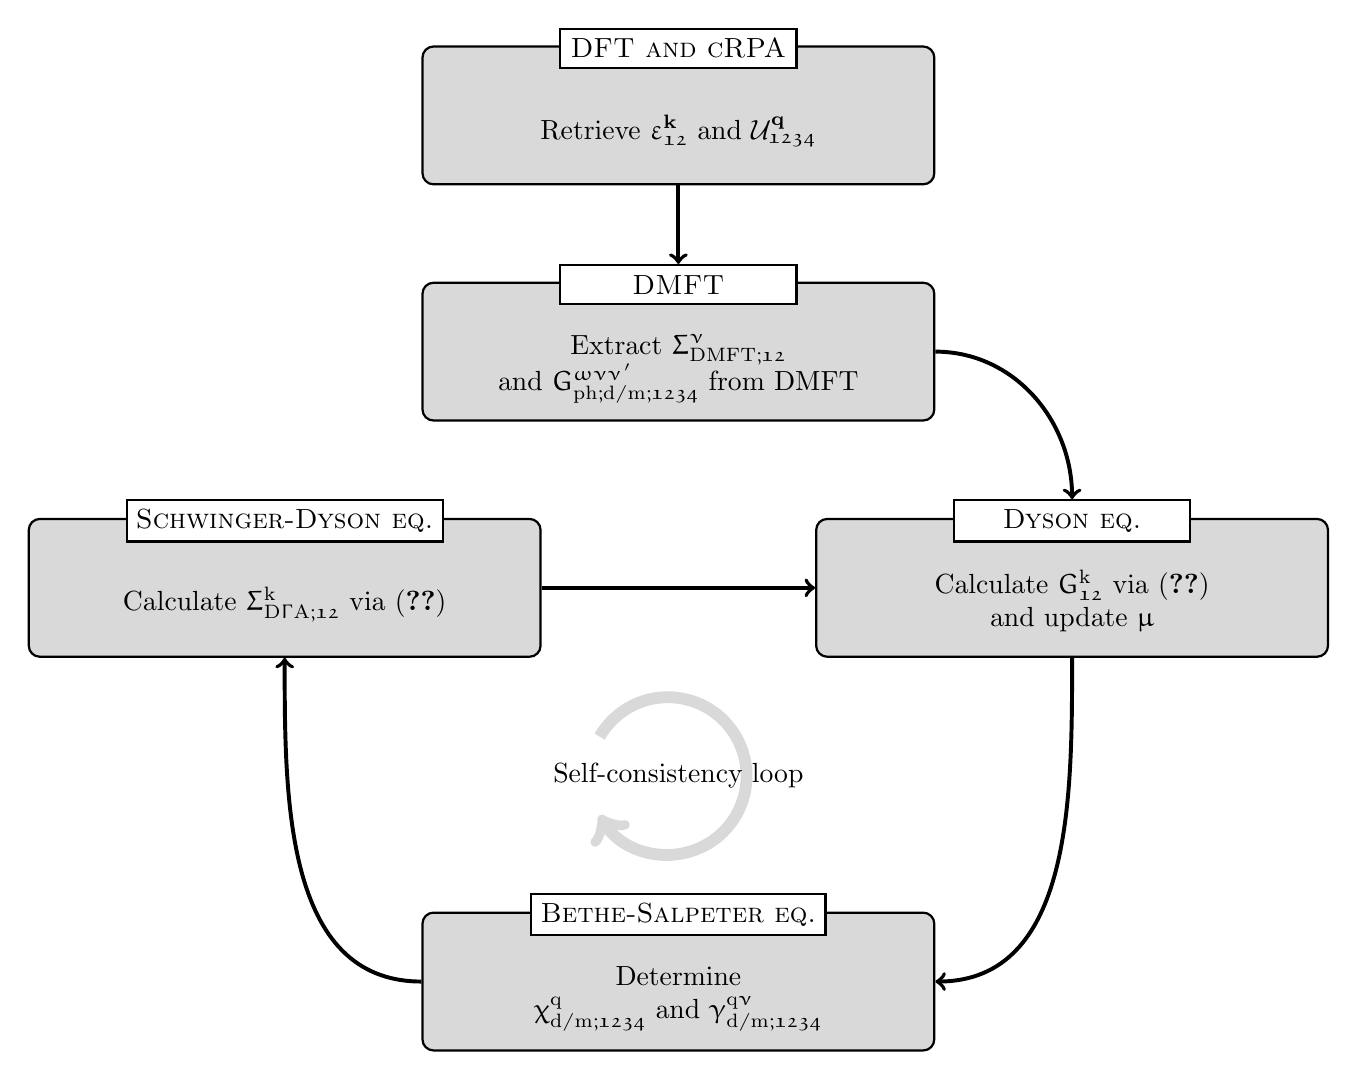
\begin{tikzpicture}	
    % Nodes
    \node (start) [box] {};    
    \node (dmft) [box] at ($(start)+(0,-3)$) {};
    \node (dyson) [box] at ($(dmft)+(5,-3)$) {};
    \node (bse) [box] at ($(dyson)+(-5,-5)$) {};
    \node (sde) [box] at ($(bse)+(-5,5)$) {};
	
	%\node (center) at ($(start.center)+(-2.5,-6)$) {};  
	%\draw[line width=7mm, draw=black!30, ->] (center) arc[start angle=150, end angle=-150, radius=2.5cm];
    
    \node (t1) at ($(start.center)+(0,-0.2)$) {Retrieve $\varepsilon_{\mathfrak{12}}^{\textbf{k}}$ and $\mathcal{U}^{\textbf{q}}_{\mathfrak{1234}}$};
    \node (t2) at ($(dmft.center)+(0,-0.2)$) {\begin{tabular}{c}Extract $\Sigma_{\text{DMFT};\mathfrak{12}}^{\nu}$ \\ and $G_{\ph;\dens/\magn;\mathfrak{1234}}^{\omega\nu\nu'}$ from DMFT\end{tabular}};
    \node (t3) at ($(dyson.center)+(0,-0.2)$) {\begin{tabular}{c}Calculate $G^{\k}_{\mathfrak{12}}$ via \eqref{eq:dyson_eq}\\ and update $\mu$\end{tabular}};
    \node (t4) at ($(bse.center)+(0,-0.2)$) {\begin{tabular}{c}Determine \\ $\chi^{\q}_{\dens/\magn;\mathfrak{1234}}$ and $\gamma_{\dens/\magn;\mathfrak{1234}}^{\q\nu}$\end{tabular}};
    \node (t5) at ($(sde.center)+(0,-0.2)$) {Calculate $\Sigma^{\k}_{\text{D}\Gamma\text{A};\mathfrak{12}}$ via \eqref{eq:sde_abinitio_dga}};
    
    \node (startheader) [header] at ($(start)+(0,0.85)$) {\scshape DFT and cRPA};
    \node (dmftheader) [header] at ($(dmft)+(0,0.85)$) {\scshape DMFT};
    \node (dysonheader) [header] at ($(dyson)+(0,0.85)$) {\scshape Dyson eq.};
    \node (bseheader) [header] at ($(bse)+(0,0.85)$) {\scshape Bethe-Salpeter eq.};
    \node (sdeheader) [header] at ($(sde)+(0,0.85)$) {\scshape Schwinger-Dyson eq.};

    \draw [flowchartarrow] (start.south) -- (dmftheader.north);
    \draw [flowchartarrow] (dmft.east) to [in=90, out=0] (dysonheader.north);  
    \draw [flowchartarrow] (dyson.south) to [in=0, out=-90] (bse.east);
    \draw [flowchartarrow] (bse.west) to [in=-90, out=180] (sde.south);
    \draw [flowchartarrow] (sde.east) -- (dyson.west);  
    
    \draw[line width=1.5mm, draw=gray!30, <-] 
        ($(dmft.south)+(-1,-5)$) arc[start angle=-150, end angle=150, radius=1cm];
    \node at ($(dmft.south)+(0,-4.5)$) {Self-consistency loop};
\end{tikzpicture}

\end{document}
